\documentclass[letter,12pt]{article}
\usepackage[T1]{fontenc}
\usepackage[utf8]{inputenc}
\usepackage{lmodern}
\usepackage{hyperref}
\usepackage[english]{babel}
\usepackage{fourier}
\usepackage[protrusion=true,expansion=true]{microtype}
\usepackage{amsmath,amsfonts,amsthm}
\usepackage[pdftex]{graphicx}
\usepackage{sectsty}								
\usepackage[svgnames]{xcolor}			
%\allsectionsfont{\centering \normalfont\scshape}	
\usepackage{fancyhdr}
\pagestyle{fancyplain}
\fancyhead{}	
\fancyfoot[L]{\small \url{http://toddvance.tech}}		
\fancyfoot[C]{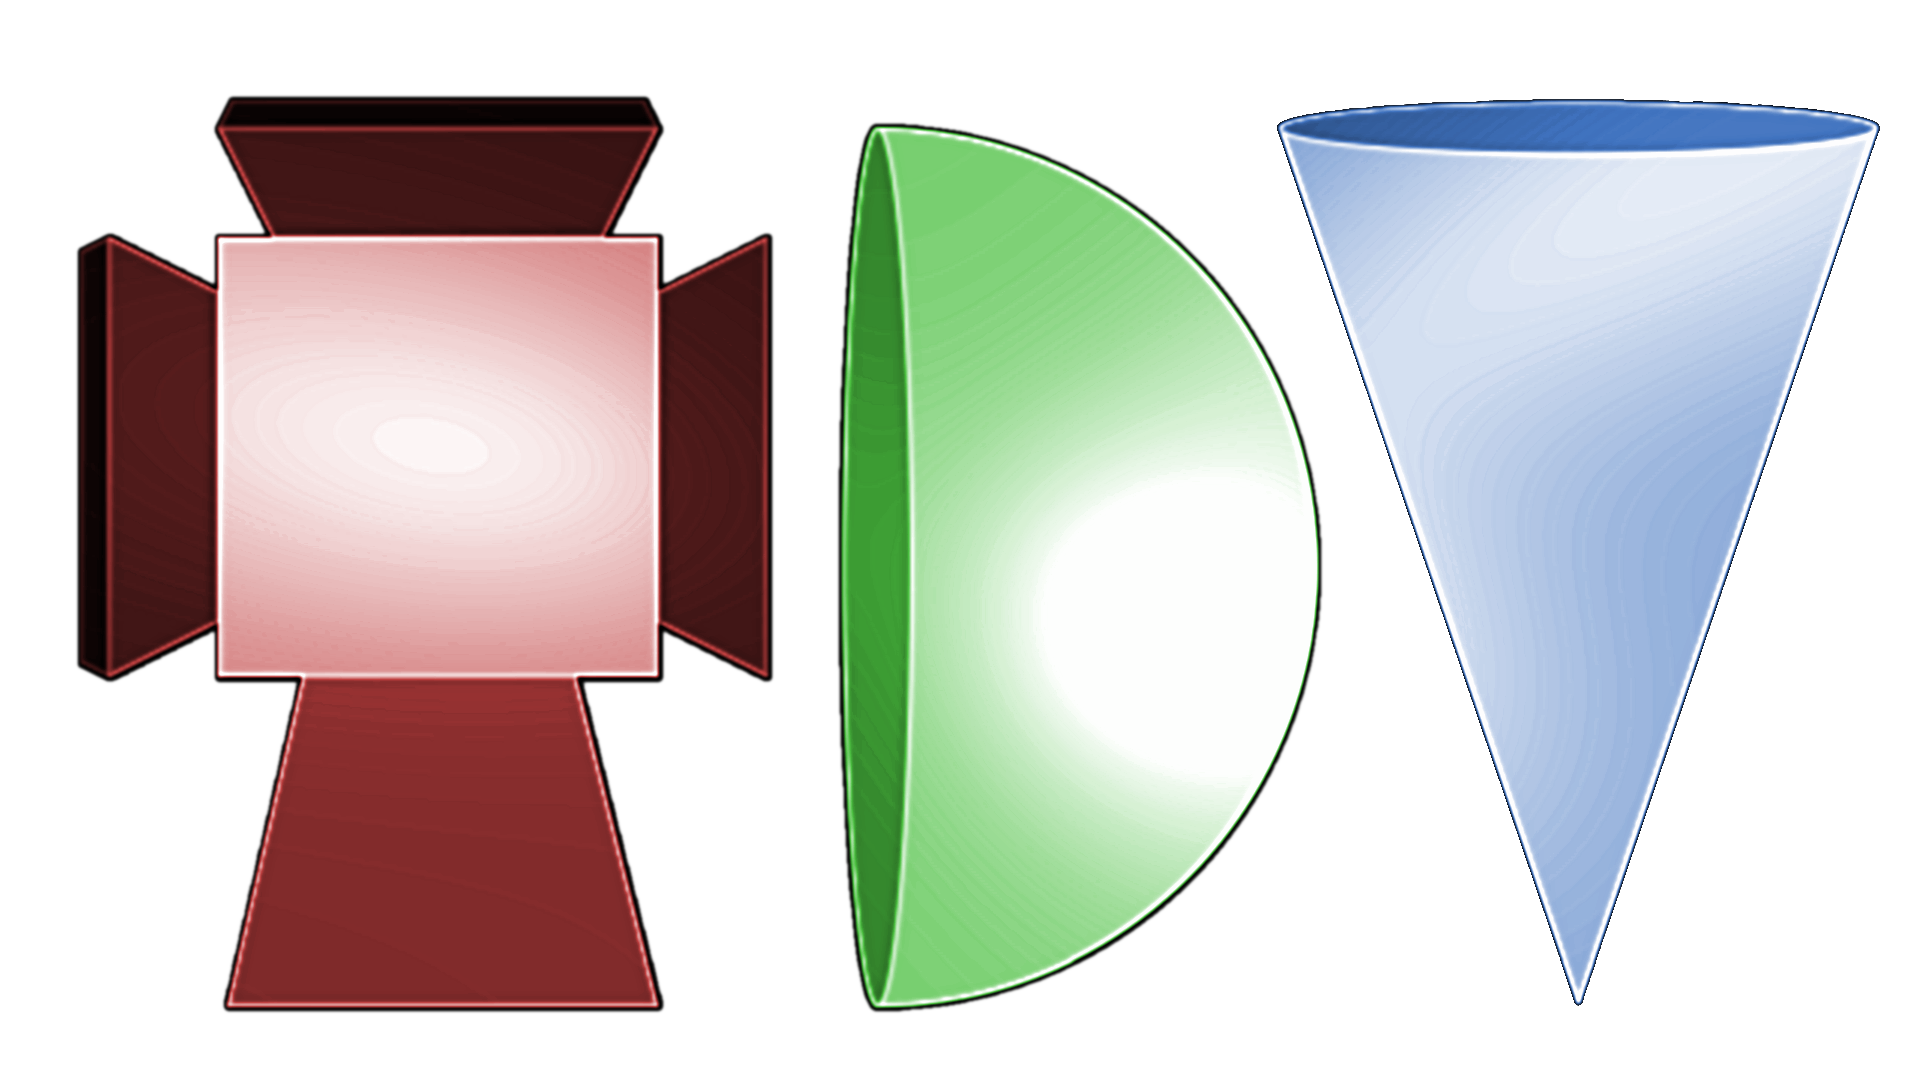
\includegraphics[width=0.5in]{Common/monogram-transparent.png}}											
\fancyfoot[R]{\thepage}								
\renewcommand{\headrulewidth}{0pt}			
\renewcommand{\footrulewidth}{0pt}
\setlength{\headheight}{13.6pt}
\newcommand{\horrule}[1]{\rule{\linewidth}{#1}} 	% Horizontal rule

\title{
		%\vspace{-1in}
		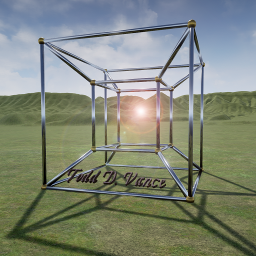
\includegraphics[width=1.5in]{Common/tdv-logo-south-branch-valley-small.png}
		\usefont{OT1}{bch}{b}{n} 
		\normalfont 
		\horrule{0.5pt} \\[0.4cm]
		\Huge Creating Real Landscapes for Unreal Engine 4 and Unity 3D\\ %%%%%%%%%%%%%% TITLE %%%%%%%%%%%%%%%
		\color{DarkGreen}
		\large How To\\[0.2cm]%%%%%%%%%%%%%%ARTICLE TYPE %%%%%%%%%%%%%%%
		\color{Blue}
		\small \textsc{It is tricky, but doable with effort and some downloading of software}\\%%%%%%%%%%%%%% TAG LINE %%%%%%%%%%%%%%%
		\color{Black}
		\horrule{2pt} \\[0.5cm]
}
\author{
		\normalfont \normalsize
       \copyright{2017 Todd D. Vance}%%%%%%%%%%%%%% COPYRIGHT %%%%%%%%%%%%%%%
        \tiny\\
\tiny        Permission is hereby granted, free of charge, to any person obtaining a copy\\[-0.3cm]
\tiny        of this software and associated documentation files (the "Software"), to deal\\[-0.3cm] 
\tiny        in the Software without restriction, including without limitation the rights to\\[-0.3cm]
\tiny         use, copy, modify, merge, publish, distribute, sublicense, and/or sell copies\\[-0.3cm] 
\tiny         of the Software, and to permit persons to whom the Software is furnished to\\[-0.3cm]
\tiny         do so, subject to the following conditions:\\[-0.3cm]
\tiny         \\[-0.3cm]
\tiny	The above copyright notice and this permission notice shall be included in all\\[-0.3cm]
\tiny	copies or substantial portions of the Software.\\[-0.3cm]
\tiny	\\[-0.3cm]
\tiny	THE SOFTWARE IS PROVIDED "AS IS", WITHOUT WARRANTY OF ANY KIND,\\[-0.3cm]
\tiny	EXPRESS OR IMPLIED, INCLUDING BUT NOT LIMITED TO THE WARRANTIES\\[-0.3cm] 
\tiny	OF MERCHANTABILITY, FITNESS FOR A PARTICULAR PURPOSE AND\\[-0.3cm]
\tiny	NONINFRINGEMENT. IN NO EVENT SHALL THE AUTHORS OR COPYRIGHT\\[-0.3cm]
\tiny	HOLDERS BE LIABLE FOR ANY CLAIM, DAMAGES OR OTHER LIABILITY,\\[-0.3cm]
\tiny	WHETHER IN AN ACTION OF CONTRACT, TORT OR OTHERWISE, ARISING\\[-0.3cm]
\tiny	FROM, OUT OF OR IN CONNECTION WITH THE SOFTWARE OR THE USE\\[-0.3cm]
\tiny   OR OTHER DEALINGS IN THE SOFTWARE.
}
\date{\today}

\begin{document}
\maketitle{}
\tableofcontents{}

%%%%%%%%%%%%%% BEGIN DOCUMENT %%%%%%%%%%%%%%%

\section{Introduction}

\begin{figure}
  \includegraphics[width=6in]{common/tdv-logo-sbv-deplorable-huge.png}
  \caption{Hypercube projected into the South Branch Valley}
  \label{fig:landscape}
\end{figure}

The logo of Figure \ref{fig:landscape} was made by placing a Blender-produced object onto a terrain generated by a heightmap.  What’s special about that terrain is it’s real...it’s where my house is.  Of course, houses, trees, roads,  and so on, are missing, and the river is “flooded out of the banks” and covers the entire flood plane, but it’s just the heightmap that’s real.  This tutorial is about getting real heightmaps from geographic data and getting them into a game engine.  The landscape of Figure \ref{fig:landscape} had a rather complex workflow, but there are easier instances as well that are covered.

\section{What is Needed?}

Unity3d accepts files in only one format: a 16 bit .raw format.  Unreal Engine 4 accepts this as well as .r16 files and 8-bit .png files.  

As for input, Terrain Party provides 8-bit .png files.  This is the easiest way to get terrains.  The downside is 8 bits per pixel means there are only 256 height levels.  Heights on earth range over 19764 meters, so each height level would be a step of up to 77 meters, which is not a very good resolution for say, a first-person character between 1 and 2 meters high.  

On the other hand the United States Geological Information System can provide full-resolution 16-bits-per-pixel files.  This allows height levels to be about 1/4 meter per step, just under a foot.  The downside here is that the files are in a proprietary format and it is not at all trivial to convert the files to 16-bit raw files.   In addition, these files are far from having world-wide coverage.  

The third options is to google around and hope to find what you need in a format you can deal with.

With this in mind, here are some setups for various levels.  Not mentioned are “obvious” needs like a web browser to download the information in the first place.

\subsection{Minimum Setup}

For the minimum setup, you need Unreal 4 engine.  It is free and can be downloaded from \url{https://www.unrealengine.com/download}, but you do have to register.

Strongly recommended is The Gimp, free, no registration needed, available at \url{https://www.gimp.org/}.

\subsection{Minimum Setup with Unity}

For the minimum-but-one setup, you need Unreal 4 engine and the Unity3d engine.  Unreal Engine 4 is free and can be downloaded from \url{https://www.unrealengine.com/download}, but you do have to register.  It is mainly used to import and export files for use in Unity3d.  Unity3d also has a free version and you need to register, and it is available from \url{https://unity3d.com/get-unity/download}.  

Strongly recommended is The Gimp, free, no registration needed, available at \url{https://www.gimp.org/}.

\subsection{Ultimate Setup}

A serious worker in terrains will want a full suite of tools.  

\begin{itemize}
\item Unreal Engine 4
\item Unity 3D
\item The Gimp
\item Up-to-date Java Runtime Environment
\item ImageJ (requires Java)
\item OSGeo4w Shell
\item L3DT 
\item Terragen
\end{itemize}

\subsection{Expert Ultimate Setup}

This is like the ultimate setup,  but even more so, and requires some expertise to set up, much less use.

\begin{itemize}
\item Unreal Engine 4
\item Unity 3D
\item Photoshop (expensive)
\item The Gimp
\item A unix-like command line (Cygwin, MinGW, Bash On Ubuntu On Windows, a Linux box, or a Mac with X-os).
\item ImageMagick (requires unix-like command line)
\item Up-to-date Java Runtime Environment
\item ImageJ (requires Java)
\item OSGeo4w Shell
\item L3DT 
\item Terragen
\end{itemize}


\section{Finding the Location}

You need the lattitude and longitude coordinates of the location you wish to model.  This is easy if the location has a name Google recognizes.  

If it’s an address, something a post office can find, like  1600 Amphitheatre Pkwy, Mountain View, CA 94043, the headquarters of Google, Inc., just enter “map  1600 Amphitheatre Pkwy, Mountain View, CA 94043” into google and click on the map that shows above the results.  The coordinates are in the address bar after the “@” sign following the address, in this case: 37.4221768,-122.0865852, where the first number is lattitude (positive for north, negative for south), and the second number is longitude (negative for west, positive for east).

If you don’t have that, try “map whatever-you-have” first and you might get lucky.  

Alternatively try “what are the coordinates of whatever-you-have”. 

For example, in this document, we shall model Armegeddon, a great place for a game battle that has hints of end times in it.

The first result from googling “what are the coordinates of Armageddon” gives you the answer: 32.5841043302,  35.1834292663

\section{Downloading a Low-Resolution Terrain}
The easiest way of proceding from here, a way that will work if you do not require too much height detail, is as follows.

Go to the website “http://terrain.party/”.  On the left-hand side, top, is a magnifying glass and hovering over it gives the tooltip “Search”.  Click the magnifying glass to get a search box.  Copy and paste  32.5841043302,  35.1834292663
 into the search box, hit Enter, and it should go right to the location.
 
 From here, you can drag the map (not the blue box marking the location) to pan, and use the mouse wheel to zoom in and out.  You can drag the blue box to move it around, but then you no longer have your chosen coordinates in the center and it might be hard to find it on the terrain as a result.  Finally, there are plus and minus icons on the top right of the window for increasing and decreasing the size of the terrain you want to download.
 
 For this purpose, zoom in as far as you can and click the “minus sign” icon until it shows 8km, the smallest terrain this site will generate.
 
When you have what you want, click the cloud icon with a downward-pointing arrow in it, near the top right to download the .zip file containing the terrain data.  It will ask for a name, and Armageddon is the obvious choice.  Hit OK and after several seconds, you get the download window from the web browser.  Save the file “Armageddon terrain.zip”, making sure it goes to a location where you can find it again (with firefox, you can find it again in the download manager, the downward arrow icon in the icon bar, or from the menubar, Tools $\rightarrow$ Downloads).

Then, find and open the zip file, and extract it to a location of your choice where you can find it again.

In this case, you get five files, a README and 4 images.  The image you want is “Armageddon Height Map (Merged).png”.  Also look at the “Armageddon README.txt” file for information about this specific terrain.

\section{Data About the Heightmap}

Make note of the following data, found in the “Armageddon README.txt” file, that you will need again:  under the “Elevation Adjustment” section, it shows that the elevations are from 31 through 378 meters.

Depending on what you do next, you probably need other data as well.  Open the “Armageddon Height Map (Merged).png” in The Gimp (some of this can be done in other programs but this howto assumes The Gimp).  You will see a grayscale image with what looks like branching structures, common for terrains in hilly areas.  Light areas are the highest places, and dark areas, the lowest places, sometimes water but not always.

Note the following information: At the very top of the window, you see the height map is 1081 by 1081 pixels.   Since the terrain is 8km by 8km, which is 8000m by 8000m, we have 8000/1081 meters per pixel, or about 7.4 meters per pixel.

Now, you need the value of the darkest pixel and the value of the lightest pixel.  To do this, click the “Windows” menu in the menubar at the top, then “Dockable Dialogs”, and look for “Histogram” and click that.

A flaw of The Gimp is for many things, it refuses to tell you exact numerical values, so you have to figure them out.  Luckily, an approximation will work for our purposes.  Below the graph are two triangles pointing up, a dark one at the bottom left of the graph above the box labeled “0”, and a light one at the bottom right of the graph above the box labeled “255”.  These can be moved and the boxes will show the values of the positions.  So, move them so the dark one is at the leftmost extent of the graph (about 9 for Armageddon), and the right one is at the rightmost extent of the graph (about 95).

This shows us that the pixel values go from 9 to 95, they correspond to the height values of 31 through 378 meters.

Thus, the range of pixels is $95 - 9 = 84$, and the range of heights is $378 - 31 = 347$.  Thus each pixel value represents a step of $347/84 = 4.13$ meters.  Finally, the maximum range of the height map is $256\cdot347/84=1057.52$ meters, or about 1058 meters.  Make note of these.

In summary, the data we have is as follows:

\textbf{Terrain: 8000m by 8000m by 347m}

\textbf{Heightmap: 1081px  by 1081px by 256 levels}

\textbf{1 pixel is 7.4 meters}

\textbf{1 level is 4.13 meters}

\textbf{256 levels is 1058 meters}

And a summary of where the data came from:

\begin{itemize}
\item 8000m by 8000m: selected at Terrain Party

\item 347m: from the README file, max height 378m minus min height 31m.

\item 1081px by 1081px by 256 levels: it’s an 8-bit .png (2 to the power of 8 is 256), and The Gimp showed it to be 1081x1081.

\item 1px = 7.4m: 8000m / 1081px

\item 1 level = 4.13m: 347m height range divided by 84 levels, where $84 = 95-9$, the 95 and 9 from the Histogram in The Gimp.
\end{itemize}

\section{Creating a Terrain in Unreal Engine 4}
For this howto, I am using  Unreal Engine version 4.14.1.  If the version number is not too far from this, the steps should be similar.  We shall create a new project without too many extras, but it can be done from an existing project too.

First, open Unreal Engine 4 and create a new Unreal project.  Under the New Project tab of the window that opens when the Unreal editor is run, click Blank under Blueprint.  Set a location for the project where you can find it again, and give it a name like “Armageddon”.  Make sure Use Starter Content is selected (so we can put a default on the landscape), as well as Maximum Quality, and you probalby want Desktop/Console, and click the green Create Project button and wait for Unreal to do its work.

\subsection{Reset the Layout}
The Unreal editor should open with some default scene.  For simplicity, we shall stick with that.  The author recommends doing the following to keep us on the same page: in the menubar at the top. click Window, then Reset Layout, and wait for the editor to restart.  This way, we know where all the windows are.  If you have a custom layout you like, save the layout (from the same Window menu item) before resetting.

\subsection{Import the Terrain}
The top left has a Modes pane.  In this pane, click the “mountains” icon to select Landscape Mode.  Create New is selected by default, so change that to Import from File.

Click the “...” button to bring up an Explorer window, and navigate to the terrain date you saved before.  Find the “Armageddon Terrain” directory (assuming that was the name you used), and in that the “Armageddon Height Map (Merged).png” file.  Click that file and click Open.

Set the landscape material to  M\_Ground\_Grass, part of the Starter Content, is a good choice, for basic grassy hills. 

Click the Fit to Data button to be sure the data is what it needs to be for the imported terrain. 

Set the scale:  because there are 7.4 meters = 740cm per pixel, the X scale and the Y scale should be 740  Because each height level is 4.13 meters or 413cm, the Z scale should be 413.  Click the “Import” button.

Finally, go back to the Place mode in the Modes panel (the icon is a cube with a lightbulb next to it).

\subsection{Adjust the Terrain}
Now, if you used the default map, the table and chairs that came with it are flying in the air above the terrain, so let us fix that.

First, let’s normalize things.  The terrain is set up so that the pivot point is at the maximum level of $256\cdot 4.13$ meters, which is about 105700cm.  The heights  go from 31m to 378m, so the terrain is too low.  If we guess the center of the terrain is around 31m, a low point, then we want the terrain to be moved 105700-3100cm, or 102600 meters from the pivot point.  So, set the Z value of the location of the landscape (make sure the landscape is selected) in the Details panel to 102600cm to start and note that now the terrain is too high.  But we are close: try lower values. Trying 100000,90000, 80000, and 70000 show that it should be between 80000 and 70000.  Now binary search: 75000 is too high.   72000 and 71000 are also too high.  70500 is just about there.  Probably better to move the table, chairs, platform, etc. slightly to a flatter place and up or down to finish the job.  In fact, selecting all the StaticMeshes, Player Start, SphereReflectionCapture, and starter\_background\_cue  in the World Outliner and moving by eye seens to work well, with the final position of the table being at -1130cm x -670cm x 172cm.

Add a Lightmass Importance Volume (in the Volumes submenu of the Place mode in the Modes panel), adjust to cover the table and chairs area, and click Build to rebuild the lighting and try it out.

\subsection{Check your Work}

Let us make sure there was no (major) error in our computations (estimates).  

In the Place mode menu, under Basic, is a Cube.  Drag one into the scene near where the table and chairs are.  The cube is 1m by 1m by 1m when the scale is at 1.

Now, our landscape should be x= 8000m by y = 8000m by z = 347m.  So, scale the cube to x= 8000 by y = 8000 by z = 347.  Set the Location z value to 0 to move it to where the terrain is and move around it, making sure that its height is about the same as the vertical extents  of the terrain, and the length and width are about the same as the terrain length and width.  We see the terrain is slightly thicker, but not much, and slightly larger horizontally as well, but not much.  I would just leave that as is.  Delete the cube.

\subsection{An Optional Tweak}

You might note the grass texture looks too big.  This is from scaling the terrain about 5x the default scale (4x in the z direction, 7x in the x and y directions, 5x is a good round number).  This can be fixed, though it takes time.

With the landscape selected, look at the Details panel on the right.  In the Landscape section is the Landscape Material.  Click the magnifying glass to bring it up in the Content Browser.

Right-click it in the Content Browser and select Duplicate.  Optionally, give it a new name.  Move the new grass material out of the Starter Content into a better location for finding it easier.  Navigate to the new location and change the Landscape texture to the newly duplicated Grass material.

Doubleclick the material to bring up the material editor.  A node diagram will appear.

Scroll around and look for the red boxes labeled “Tex Coord”.  There are 5 of them, and all 5 need to be changed.  There is another red box that says PixelDepth, but that need not be changed.

Click on one of them, and look at the Details panel to the left, in the section Material Expression Texture Coordinates.  There are two boxes, UTiling an VTiling.  Just multiply those values by 5.  Thus, the topmost box has .75 as the value for each, so change both values to $.75\cdot5=3.75$.  The second box from the top has both values at .5, so change them to 2.5.   The third box from the top has values of 0.05, so change then to 0.25.  The fourth box has values of 1.  Change them to 5.  The fifth box also has values of 1, so change them to 5.

Click the green arrow in a blue circle icon at the top left that is labeled Apply, and then click the blue diskette icon to the left of that to save.  Close the Material Editor window and rebuild the level lighting and look at the effect.

\section{Move the Unreal 4 Terrain to Unity 5}
Specifically, I am using Unity version 5.5.0f3.  The steps “should” work on any unity 5, version 5.5 or higher, and perhaps on earlier versions if not too much earlier, though the details will likely change.

\subsection{Create a Raw File from the .png File with Unreal Engine 4}
Unity3d likes 16 bit raw files, not .png files.  If you have software to do that, go ahead (more about this in later sections).  But if not, and you have Unreal 4...well, you have software to do that!  Follow the previous steps to import your terrain into Unreal 4 (you can even cheat and skip the scaling part, just import the heightmap).

Return to Landscape mode (mountain icon) in the Modes panel, make sure the Sculpt icon is selected, and right click the Heightmap under the Target Layers section.  One option is to Export to File.  Click that, select Heightmap .raw/.r16 files, and optionally change the name and/or directory (in fact, change the suffix to .raw, because that’s what Unity likes), and click “save”.  You now have your raw file! 

\subsection{Create an empty Unity3d Project}

\begin{figure}
  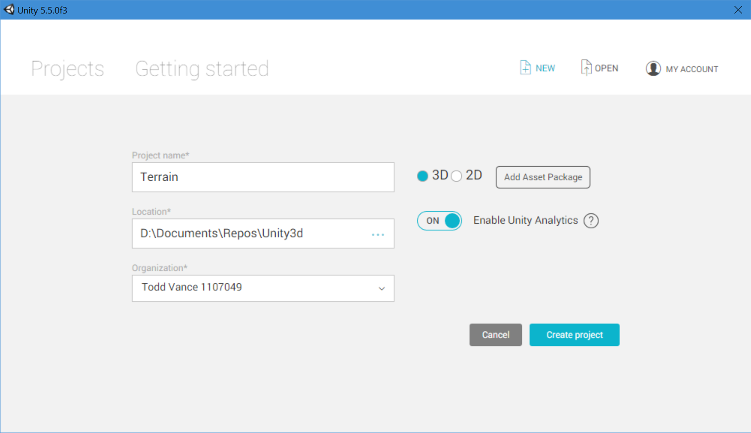
\includegraphics[width=6in]{RealLandscape/projects.png}
  \caption{New Terrain Project}
  \label{fig:projects}
\end{figure}

\begin{enumerate}
\item Open Unity.
\item When the Projects (or Getting Started) window opens up, click the dog-eared sheet of paper with a plus sign in it (“New”) to create a new project.
\item Name the project Terrain, and make sure “3D” is selected.  No asset packages need be selected, and Unity Analytics are your choice.  Make sure the Location field points to a convenient directory that you can find again.  See Figure \ref{fig:projects}
\item Click the bluish-green “Create Project” button.
\item When the Unity IDE window opens, look for the Layout dropdown at the top right, click it and select Default.
\end{enumerate}

\subsection{Create a Terrain}
\begin{enumerate}
\item At the top left of the screen, at the top of the  Hierarchy pane, is a Create dropdown.  Click Create $\rightarrow$ 3D Object $\rightarrow$ Terrain.  A new terrain will show in the scene.
\item Select the Terrain in the Hierarchy pane and note that it appears in the Inspector pane on the right.
\item In the Terrain component, there is a row of icons.  Click the rightmost Cog icon (Terrain Settings).  The Terrain Settings view will now show in the Inspector.
\item Now, click the “Import Raw...” button in the Heightmap section, at the bottom of the Terrain component, just above the Terrain Collider component.
\item An explorer window will open.  You now need to navigate to where you saved the heightmap file. Select the .raw file you had just saved.
\item Next a configuration popup will appear.  Most items can be left as default, but make sure the dimensions are 8000 by 8000 horizontally, and 1058 (256 times 3.14, about) vertically.  Note that in Unity, the Y value, not the Z value, is the vertical value, and Unity3d units are in meters, not centimeters.
\end{enumerate}

\subsection{Check your Work}

Let us make sure there was no (major) error in our computations (estimates).  

From the GameObject menu in the menubar, select 3D Object and then Cube.

Now, our landscape should be x= 8000m by y = 347m by z = 8000m.  So, scale the cube to x= 8000 by y = 347 by z = 8000. Put it at about 4000 by 150 by 4000, near the center of the landscape.  Check that the dimensions of the landscape are similar to the dimensions of the cube.

It does fit, but the landscape texturing doesn’t.  Looking at the Inspector with the Landscape selected shows that it thinks the heightmap resolution is 2049, close to twice what it actually is.  So, only one-fourth of the map has hills and the rest is plain.  Changing the heightmap resolution doesn’t seem to work in Unity 5.5.0f3 (it forces you to reimport, in fact).   

The solution would be to scale the raw image file up to 2049 by 2049 that Unity3d will accept.  This requires software that can handle the 16-bit raw image format (like Photoshop or ImageJ).  

Another solution is to change the width and height of the terrain in the Inspector to 16000 by 16000 and ignore the bad parts of the terrain.

Delete the cube when you reach something satisfactory.

Next, we would like to add a realistic material to the terrain.  In the menubar, under assets,  click Import Package, then select Environment.  Go ahead and import it all.

When this is done (it will take a minute or so), click the paintbrush icon about the middle of the row of icons that contain the cog icon.  Click Edit Textures, then Add Texture.  It will let you select an albedo texture (an ordinary image texture) and a normal texture.  Click Select for albedo and select Grass Hill Albedo from the choices (this is from the Environment package).  It does not come with a corresponding Normal texture, though you can try the muddy normal to see if it looks reasonable or not.  Optionally experiment with things like the smoothness value.

Reselect the cog icon to prevent accidental painting of the landscape.

Optionally add detail and trees.  The asset pack also has some things like water you can add.

You may want to move the camera to a more reasonable place (like 4000, 155, 4000) and try running the game to see how it looks.

Save the scene when satisfied. 

\section{Expert Topic: Using US GIS Data}

This process is not simple and requires multiple steps in multiple downloaded software components.  The Expert Ultimate Setup is strongly recommended for this.  

\subsection{Find and Download the File}

The data is currently at the following page: 
\url{https://viewer.nationalmap.gov/basic/?basemap=b1&category=ned,nedsrc&title=3DEP%20View}.%}
However this site does move from time to time.  You may need to google for “usgs digital elevation models 3dep”  (“3dep” being the current name for the product; it used to be “ned”).

This is limited to  (most of) the US, so we shall work with a rugged area of the US.

Doing a Google search for “what are the coordinates of Mt. St. Helens” gives the result 46.1914, -122.1956.  Navigating to the viewer.nationalmap.gov site above and pasting these coordinates into the “Search location” box and clicking the blue “Go” button brings up a topographical map with an obvious volcano in the center.

Clicking the “Find Products” link on the popup at the volcano gives 3 results.  Clicking the “Results” links to the left gives several choices, of which the best appears to be  “USGS NED n47w123 1/3 arc-second 2013 1 x 1 degree ArcGrid”.

Click “Download” to get the zip file.  It will take a few minutes.  This file is 1 degree by 1 degree so it covers a fairly large area, and Mt. St. Helens is not in the exact center.

However, taking a screenshot of the map with the superimposed thumbnail of the image will help one find this information again.

When the download finishes, extract the zip file to a location you can find, perhaps the same place where the screenshot is saved.

\subsection{Convert the Files to a Usable Image}

The “readme.pdf” file explains what file formats might be found in the folder (on Page 2). In this case, we have a folder called grdn47w123\_13, which is something called “ARCGRID” format.  It may also have a GRIDFLOAT format or an IMG format.  All three formats are proprietary and not well-supported by most software.  However the same program “gdaltranslate”, part of the OSGEO4W shell, will probably work on all three formats.

Looking in the grdn47w123\_13, we see the most likely candidate for the raw data is the w001001.adf file, since it is the largest.  Googling for ARCGRID .adf format shows that GDAL software (part of OSGEO4W) can handle this.

So, run the OSGEO4W shell, and change to the directory grdn47w123\_13.  Type “gdaltranslate -ot Int16 w001001.adf output.tif” and it will produce a .tif file from the .adf file: “heightmap.tif”.

Now, open this file in ImageJ (which handles Int16 .tif files just fine), and check that it looks reasonable.  

Use ImageJ to save as type .png (heightmap.png).  This is 16-bit png, which Unreal accepts.

Test the heightmap by opening it in Unreal.  Size adjustment (scaling and cropping) may be needed to get it to work in Unity.  Suggest exporting from Unreal because the “.raw” format exported y ImageJ doesn’t seem to be right for Unity.  You might also try L3DT or Terragen and see if that converts the files properly.

\end{document}